\chapter{The Dataset Management Framework}
\label{sec:generic_dataset}
In the initial phase of this thesis, we did not know what data characterized the collected examples. To overcome this uncertainty, we develop \textit{generic-dataset}\footnote{The generic-dataset repo: \url{https://github.com/micheleantonazzi/generic-dataset}.}, a configurable framework that automatically generates the code and the necessary classes to manage a dataset of any kind. This is possible using the \textit{meta-programming} paradigm offered by Python. Meta-programming is a technique in which computer programs have the ability to generate new code, create other programs, and modify their internal structure while running. This allows programs greater flexibility to efficiently handle new situations without recompilation. 

In Python, the meta-programming paradigm is implemented using \textit{decorators} and \textit{meta-classes}. A decorator allows programmers to modify the behavior of functions or classes. In other words, a decorator wraps an entity into a function in order to extend the behavior of the wrapped function or class, without permanently modifying it. The meta-classes, otherwise, represent a further implementation of meta-programming. In Python, everything is an object and classes are objects as well. A class in Python must have a type and it is an instance of another super-type, called meta-class. In simple terms, a meta-class is the definition of a class. The default meta-class which is responsible for making classes is called \textit{type}. Fig. \ref{fig:metaclass} visually explains the concept just reported: an object is an instance of a class and a class is an instance of a meta-class.

\begin{figure}[h!]
	\centering
	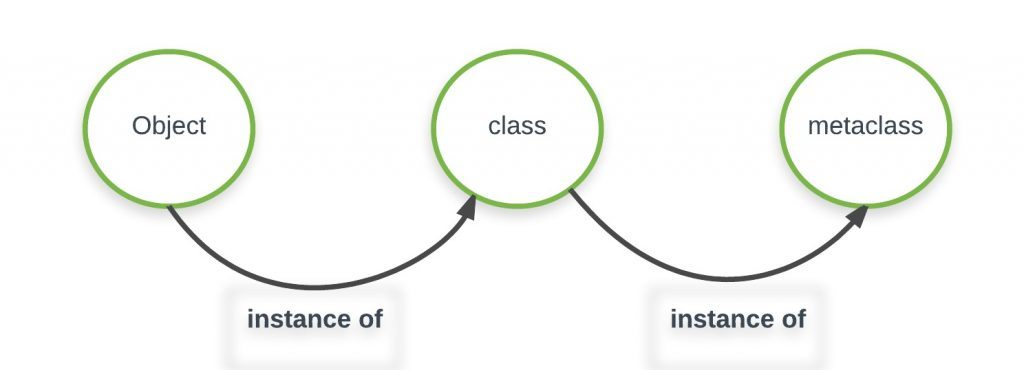
\includegraphics[width=\textwidth]{images/metaclass-hierarchy.jpeg}
	\caption{The hierarchy of objects, classes and meta-classes.}
	\label{fig:metaclass}
\end{figure}

Thanks to meta-programming, the programmer can write his own custom meta-classes to modify the way from which classes are generated by performing extra actions or injecting code. By exploiting this principle, the \textit{generic-dataset} framework offers an intuitive API that creates a custom class to model a particular examples' type of a generic dataset. To do this, this API, implemented by a \textsf{SampleGenerator} object, creates a meta-class according to the directions of the programmer, that defines the final desired class to deal with precise dataset's examples. In the constructor of \textsf{SampleGenerator}, the user specifies the name of the generated sample class and the label set. In this way, both regression or classification problems can be modeled. In a regression problem, the labels are real numbers and the label space is typically infinite. In this first case, the label set passed to the constructor must be empty. Otherwise, in a classification problem, the label set must contain all the possible labels that an example can assume. The programmer can also add data fields to the final generated class, specifying their name and type. In this case, the framework automatically generates useful methods to manipulate the custom fields (like getters and setters functions). Furthermore, the user can add custom methods to the final class in order to manipulate the example's fields. Finally, using the \textsf{generate\_sample\_class} method, \textsf{SampleGenerator}, the user obtains the generated custom class (which is an instance of the configured meta-class) which models a specific type of example. The instances of the generated class, that deal directly with the examples, are thread-safe. The generated class automatically implements this feature by assigning a lock to each data field. Then, each method is decorated with a function that acquires the locks of the fields used within each method before execution and then releases them. Also, the custom methods can be synchronized by specifying the name of the used fields.

Despite we did not know the exact final composition of our dataset, surely we will deal with image manipulation. To address this requirement,  \textit{generic-dataset} offers a useful utility to manipulate RGB images, that in Python are commonly stored in NumPy arrays. This utility, implemented by the \textsf{DataPipeline} class, generates an elaboration pipeline to modify a NumPy array. A pipeline consists of a series of operations performed consecutively that can be executed in CPU or in GPU according to the programmer's needs without changing the code. This is possible using CuPy\footnote{The CuPy web page: \url{https://cupy.dev/}.}, an open-source array library for GPU-accelerated computing with Python. The CuPy's interface is highly compatible with NumPy, allowing to write agnostic programs which can be executed in CPU or GPU by replacing the engine (NumPy or CuPy), without any code change. A pipeline can be customized by adding functions to modify the initial array and then executed using the \textsf{run} method. If the \textsf{use\_gpu} flag is set as \textsf{False}, the pipeline is synchronously executed in the CPU. Otherwise, if such flag is \textsf{True}, the operations are asynchronously performed by the GPU, so the user must synchronize the two elaboration units through the \textsf{get\_data} method. This mechanism is integrated into the class generated by \textsf{SampleGenerator}. It offers the possibility to automatically create an elaboration pipeline for the fields of the generated sample class. In addition, pipelines are protected with a dedicated lock which prevents data access and modification when during the execution of the correspondent pipeline.

The \textit{generic\_dataset} framework provides a mechanism to manage the dataset's persistence. It automatically organizes the folder hierarchy to store and organize the dataset and offers the necessary methods to save and load the examples. The classes generated by \textsf{SampleGenerator} are sub-type of \textsf{GenericSample} class, which provides a utility method to manage an example instance class of any kind. When the programmer adds a new field to the generated class, it must specify if it belongs to the dataset and, if so, it must provide the necessary functions for saving and loading such data type to the disk. The dataset folder hierarchy is organized as follows. The main directory is divided into sub-folders, that could specify different data categories or different moments in which the data are collected. Then, for a classification problem, the samples are divided into another level of sub-directories according to their label. Otherwise, in a regression task, the samples are saved in the same directory and the labels are stored in a dedicated file. Finally, the examples' fields are saved in different folders and the files inside them are named to reconstruct the acquisition order. More precisely, the file name contains two counters: the relative count and the absolute count. The first indicates the example's number based in its label's folder while the latter is the absolute count of the sample over all dataset. For a regression problem, these two values are equal because all examples belong to the same directory. Fig. \ref{fig:structuredataset} visually explain the folder hierarchy of a classification (Fig. \ref{fig:structureclassification}) and a regression (Fig. \ref{fig:structureregression}) problem. The entire dataset can be managed by an instance of \textsf{DatasetManager} class, while each folder at the first nesting level is controlled by an instance of \textsf{DatasetFolderManager}.

\begin{figure}[h!]
	\centering
	\begin{subfigure}[b]{0.5\textwidth}
		\dirtree{%
			.1 MAIN\_DATASET\_FOLDER.
			.2 FOLDER\_1.
			.3 0.
			.4 FIELD\_1.
			.5 field\_name\_rc\_ac.
			.5 field\_name\_rc\_ac.
			.5 \vdots.
			.4 FIELD\_2.
			.5 \vdots.
			.3 1.
			.4 FIELD\_1.
			.5 \vdots.
			.4 FIELD\_2.
			.5 \vdots.
			.2 FOLDER\_2.
			.3 \vdots.
			.2 \vdots.
		}
		\caption{}
		\label{fig:structureclassification}
	\end{subfigure}
	\begin{subfigure}[b]{0.4\textwidth}
		\dirtree{%
			.1 MAIN\_DATASET\_FOLDER.
			.2 FOLDER\_1.
			.3 LABEL.
			.4 label\_rc\_ac.
			.4 label\_rc\_ac.
			.4 \vdots.
			.3 FIELD\_1.
			.4 field\_name\_rc\_ac.
			.4 field\_name\_rc\_ac.
			.4 \vdots.
			.3 FIELD\_2.
			.4 field\_name\_rc\_ac.
			.4 field\_name\_rc\_ac.
			.4 \vdots.
			.2 FOLDER\_2.
			.3 \vdots.
			.2 \vdots.
		}
		\caption{}
		\label{fig:structureregression}
	\end{subfigure}
	\caption{The structure of a binary classification dataset (a) and a regression dataset (b). The files' names are are lowercase, where \textsf{rc} indicates the relative count of an example inside its label's folder, and \textsf{ac} represents the example's absolute count. }
	\label{fig:structuredataset}
\end{figure}